% This file was created with tikzplotlib v0.10.1.
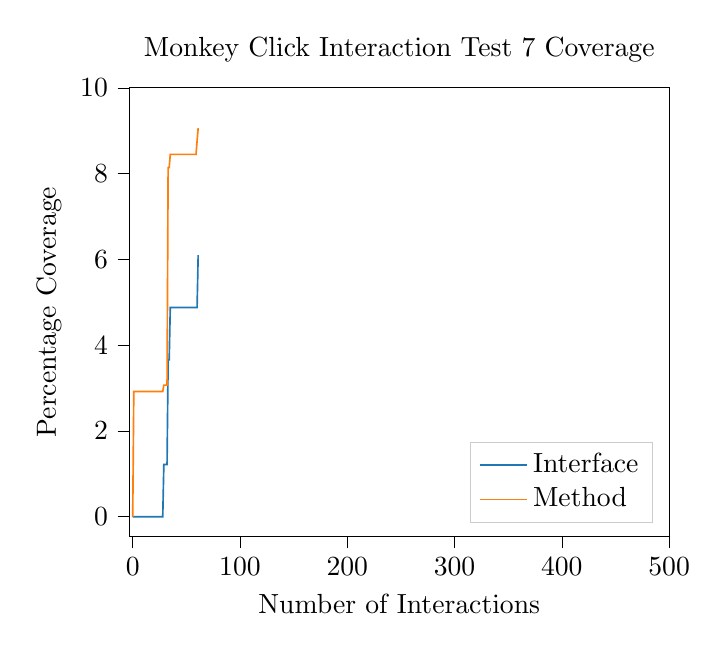
\begin{tikzpicture}

\definecolor{darkgray176}{RGB}{176,176,176}
\definecolor{darkorange25512714}{RGB}{255,127,14}
\definecolor{lightgray204}{RGB}{204,204,204}
\definecolor{steelblue31119180}{RGB}{31,119,180}

\begin{axis}[
legend cell align={left},
legend style={
  fill opacity=0.8,
  draw opacity=1,
  text opacity=1,
  at={(0.97,0.03)},
  anchor=south east,
  draw=lightgray204
},
tick align=outside,
tick pos=left,
title={Monkey Click Interaction Test 7 Coverage},
x grid style={darkgray176},
xlabel={Number of Interactions},
xmin=-3.05, xmax=500,
xtick style={color=black},
y grid style={darkgray176},
ylabel={Percentage Coverage},
ymin=-0.453, ymax=10,
ytick style={color=black}
]
\addplot [semithick, steelblue31119180]
table {%
0 0
1 0
2 0
3 0
4 0
5 0
6 0
7 0
8 0
9 0
10 0
11 0
12 0
13 0
14 0
15 0
16 0
17 0
18 0
19 0
20 0
21 0
22 0
23 0
24 0
25 0
26 0
27 0
28 0
29 1.22
30 1.22
31 1.22
32 1.22
33 3.66
34 3.66
35 4.88
36 4.88
37 4.88
38 4.88
39 4.88
40 4.88
41 4.88
42 4.88
43 4.88
44 4.88
45 4.88
46 4.88
47 4.88
48 4.88
49 4.88
50 4.88
51 4.88
52 4.88
53 4.88
54 4.88
55 4.88
56 4.88
57 4.88
58 4.88
59 4.88
60 4.88
61 6.1
};
\addlegendentry{Interface}
\addplot [semithick, darkorange25512714]
table {%
0 0
1 2.92
2 2.92
3 2.92
4 2.92
5 2.92
6 2.92
7 2.92
8 2.92
9 2.92
10 2.92
11 2.92
12 2.92
13 2.92
14 2.92
15 2.92
16 2.92
17 2.92
18 2.92
19 2.92
20 2.92
21 2.92
22 2.92
23 2.92
24 2.92
25 2.92
26 2.92
27 2.92
28 2.92
29 3.07
30 3.07
31 3.07
32 3.07
33 8.14
34 8.14
35 8.45
36 8.45
37 8.45
38 8.45
39 8.45
40 8.45
41 8.45
42 8.45
43 8.45
44 8.45
45 8.45
46 8.45
47 8.45
48 8.45
49 8.45
50 8.45
51 8.45
52 8.45
53 8.45
54 8.45
55 8.45
56 8.45
57 8.45
58 8.45
59 8.45
60 8.76
61 9.06
};
\addlegendentry{Method}
\end{axis}

\end{tikzpicture}
